
% ------------------------------------------------------------------------------------------------------------------------------------------------
\chapter{System design}
\label{chap:system-design}

The system, from here to be referred to by the name ''\textit{Oculus}'', is designed with an asynchronous as well as distributed aproach in mind. In order to achieve high asynchrononisity between obtaining new reference data, and running jobs such as ''\textit{compare video1 with the reference database}'', the system was split into two primary components: 

\begin{itemize}
  \item \textbf{loader} -- which is responsible for obtaining more and more reference material. It persists and initially processes the videos, as well as any related metadata. In a real system this reference data would be provided by partnering content providers, yet for this 
  \item \textbf{analyser} -- which is responsible for preparing and scheduling job pipelines for execution on top of the Hadoop cluster and reference databases.
\end{itemize}

To further illustrate the separate components and their interactions Figure \ref{fig:system-overview} shows the different interactions within the system.

\begin{figure}[hc!]
 \centering
  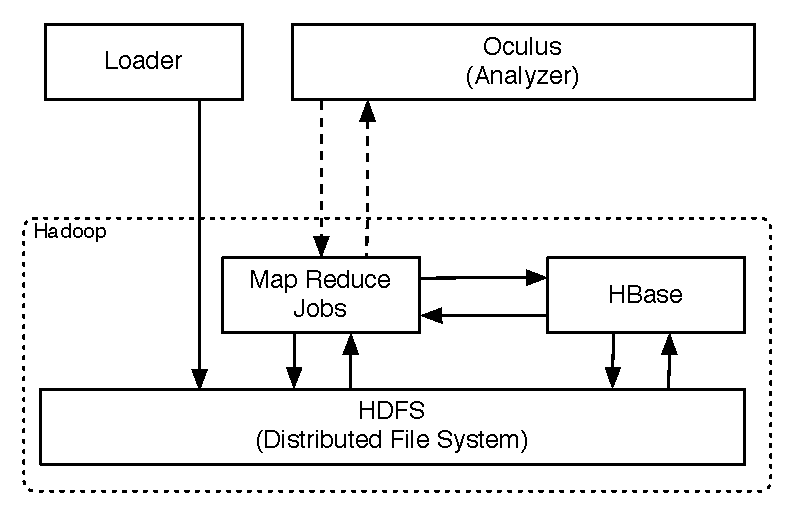
\includegraphics[scale=0.9]{./diagrams/high-level-system.pdf}
  \caption{High level overview of the system's architecture}
  \label{fig:system-overview}
\end{figure}

% ------------------------------------------------------------------------------------------------------------------------------------------------
\section{Loader}
\label{sec:loader-basics}
The Loader component is responsible for obtaining as much as possible ''reference data'', by which video material from sites such as \textit{youtube.com} or video hosting sites is meant. Please note that for the sake of this thesis (and legal safety) the downloaded content was limited to movie trailers (which are freely available on-line) as well as series opening, ending sequences.

While the Loader system will be referred to from here on in singular, it should be noted that in fact there are multiple instances of it running in the cluster. Thanks to the use of Akka's \cite{akka-docs} Actor Model abstractions (and \textit{remoting} module \cite{akka-remoting}), in which the physical location of an Actor plays is of no importance -- meaning, that the receiving Actor does not have to be on the same host as the sending Actor.

\subsection{Types of Actors used in the system}
\label{sec:types-of-actors}

The system consists of 4 types of Actors each of which has multiple instances which are spread out on many nodes in the cluster. Some tasks can only be sent to local Actors (any work requiring an already downloaded file), but messages related to crawling and initially downloading the video material can be spread throughout the cluster. 

The following Actor descriptions are aimed at explain

will now briefly describe the different Actor roles that exist in the system and then explain the interactions between then on an example.

\begin{itemize}
  \item \textbf{YouTubeCrawlActor} -- is capable of fetching and YouTube websites and generate Messages triggering
                                    either further crawling of ''related video sites'' (\verb|Crawl(siteId: String)|) or downloading of the 
                                    currently accessed video (by sending a \verb|Download(movieId)| message),
    \subitem  \textbf{receives:}
      \subsubitem 1 -- \verb|Crawl(siteId: String)| message
    \subitem  \textbf{sends:}
      \subsubitem 0 or n -- \verb|Crawl(siteId: String)| - where n is the number of ''related video'' links found on the site. 
                                                           If crawling is turned off, no messages will be sent.

  \item \textbf{DownloadActor} -- is responsible for downloading the movie from youtube in it's original format (in the presence of many formats, 
                                the highest quality file will be downloaded). This Actor decides if a video is legal to download or not, because it also
                                obtains the movie's metadata -- only trailers and opening sequences of series are downloaded during for the sake of this 
                                thesis.
                                
  \item \textbf{ConversionActor} -- is responsible for converting the downloaded video material into raw frame data (bitmaps).
    \subitem  \textbf{receives:}
      \subsubitem \verb|Convert(localVideoFile: java.util.File)| -- This message must come from a local Actor, since the path refers to the local file system.
    \subitem  \textbf{sends:}
      \subsubitem \verb|Upload(framesDirectory: java.util.File)| -- when the finished converting to bitmaps, it will send and \verb|Upload| message to one of the\verb|HDFSUploadActors|, pointing to the directory where the output bitmaps have been written.
                                                                    
  \item \textbf{HDFSUploadActor} -- is responsible for optimally storing the sequence of bitmaps in Hadoop. This includes converting a series of 
                                  relatively small (around 2MB per frame) files into one Sequence File on HDFS. Sequence Files and the need for their use
                                  will be explained in detail in section \ref{sec:sequence-files}.
  \subitem \textbf{receives:}
    \subsubitem \verb|Upload(framesDirectory: java.util.File)| -- pointing to a local directory where the bitmap files have been stored.
                                                                 This message must come from a local actor, since the path refers to the local file system.
    \subitem  \textbf{sends:}
      \subsubitem 0 or 1 -- \verb|ConfirmUpload(localFile: java.util.File)| -- sent back to the sender that requested the video to be uploaded.
\end{itemize}

Using these Actors and protocols between them, the application is able to progress safely without the possibility of getting stuck in a dead (or live) lock. 

While discussing there protocols one should also mention that the messages that can be received and sent by Actors are not possible to verify using static typing -- an Actor can receive a message of ''Any'' type, and in case of not being able to act upon it - it will drop the message, but the delivery still happens.
This is an inherent property of the Actor Model of concurrency -- which is why in such systems explaining the flows of mesages and Actors present in the system is of such importance. Having this in mind, the next Section (\ref{sec:obtaining-reference-material}) will focus on explaining one such message flow within the system.

% -------------------------------------------------------------------------------------------------------------------------------------------------
\subsection{Obtaining reference video material}
\label{sec:obtaining-reference-material}
This section wills discuss the process of obtaining video material by the Loader subsystem, as well as explain which parts can be executed on different nodes of the cluster. The Figure \ref{fig:high-level-loader} should help in understanding the basic workflow.

\begin{figure}[ch!]
  \centering
  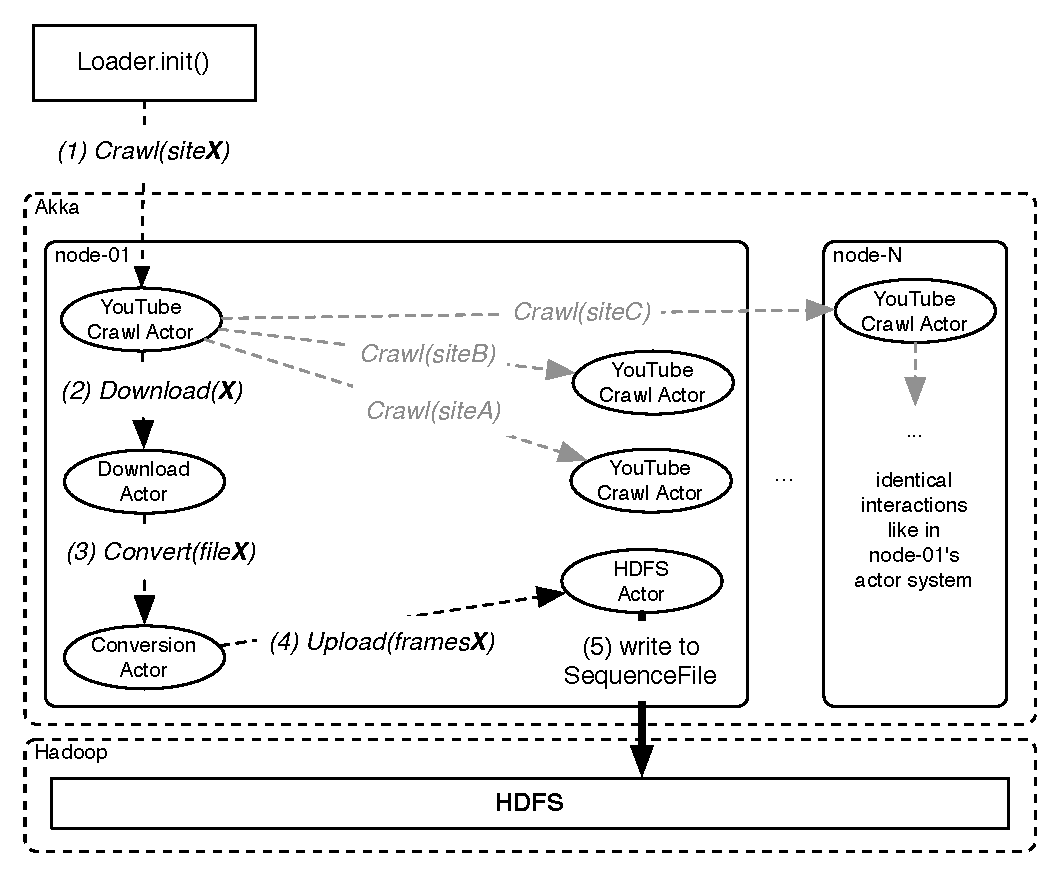
\includegraphics[scale=0.9]{./diagrams/loader-high-level.pdf}
  \caption{Overview of messages passed within the Loader's actor system. Greyed out messages are also sent, but are not on the critical path leading to obtaining material from \textit{siteX} into HDFS.}
  \label{fig:high-level-loader}
\end{figure}

\subsubsection{Step 1 - \textit{Crawl} messages}
The initiating message for each flow within the Loader is a \textit{Crawl(siteUrl)}, where siteUrl is a valid youtube video url.
The receiving YouTubeCrawlActor will react to such message by fetching and extracting the related video site urls and will forward those using the same kind of \textit{Crawl} messages. The second, yet most important, reaction is sending a \textit{Download(movieId)} message to an instance of an DownloadActor -- it  can reside on any node in the cluster, which allows us to spread the down-link utilisation between different nodes in the cluster.

It is worth pointing out that the receivers of these messages can be \textit{remote} Actors, that is, can be located on a different node in the Cluster than the sender. In order to guarantee spreading of the load among the many actors within the system (across nodes in the cluster), a routing strategy called ''Smallest Inbox Routing'' was used. This technique uses a special ''Router Actor'' which is responsible for a number of Routees (target Actors), and decides to deliver a message only to the Actor who has the smallest amount of messages ''not yet processed'' (which are kept in an Queue called the ''Inbox'', hence the strategy's name).

\subsubsection{Step 2 - \textit{Download} messages}
In the second step an \textit{YouTubeDownloadActor} instance receives a message asking it to download a movie.
It does so by invoking the native app \textit{youtube-dl}, which is an open source program specialised in downloading movies from YouTube.
Other than the video file (in an open source format) we also download a metadata description during this step, such metadata includes for example the date of publication, author, title and description of the movie. From this message including, all messages will be routed only to Actors local to the current node, because messages include \textit{File} objects, pointing to locations on-disk.

The metadata is then used to determine if it can be used in the context of this work, as only movie trailers and and opening / ending sequences are downloaded into the Oculus system. If the content is OK to use, the Actor sends an \textit{Convert(movieLocation)} message to an instance of \textit{ConversionActor}.

\subsubsection{Step 3 - \textit{Convert} messages}
The next step is executed by an instance of an \textit{ConversionActor} recieving an \textit{Convert(file)} message from another (local) Actor. The conversion phase will extract raw frame data from the incoming movie, and write those as plain bitmaps (not compressed) to files (one per each frame) into a specified target directory. The reason for not using a compressed lossless image format here is that all algorithms that the system will be dealing with later on are dealing with the raw image data, so we can avoid having to go over uncompression phases each time we will process a frame. Having that said, the storage format used for storing these files on HDFS provides build in compression (if enabeled), and it should be preferred in this case as it is transparent for the application, easing development of Map Reduce jobs in the Analyser system immensely.

The conversion from movie to raw bitmaps is performed by running an native application called \verb|ffmpeg| \cite{ffmpeg} instance (an de facto standard tool for such media operations), by forking a process from within the Actor. The CPU usage of running this extraction process easily reaches 100\% of the available resources, which is why the number of Conversion Actors per node is limited to only 1 per node, allowing ffmpeg to consume all available resources and finish extracting the data sooner. The actor will block until the process completes, and will then continue by sending an \textit{Upload(bitmapDirectory)} message to one of the \textit{HDFSUploadActors}.

\subsubsection{Step 4 \& 5 - \textit{Upload} messages}
The last step is an \textit{HDFSUploadActor} recieving an \textit{Upload(bitmapDirectory)} message which triggers it to connect to HDFS and start writing the bitmap data contained in the given directory to HDFS. The format of the generated data is as previously mentioned one file per frame of video, which averages around 2MB (depending on the movie resolution).

In this step the important part is that it does not write these files 1:1 onto HDFS, but instead writes into one file, using a hadoop specific storage format called ''Sequence File'', which allows for more efficient storage and latter retrieval of this data. Sequence Files, the need and benefits gained by using them as storage format for ''frame by frame'' data will be discussed in Section \ref{sec:sequence-files}.

This write terminates the operations performed on one movie by the Loader. All other operations will be performed by the Analyzer by running Map Reduce jobs on Sequence Files prepared in the above flow.

\subsection{Loader design summary}
As was explained in the previous sections the Loader is designed as fully asynchronous system, composed of Actors performing very specific tasks. All communication between the Actors is implemented as message passing, which provides so-called ''location transparency'' between the Actors -- this property has been utilised to spread the work-load between multiple nodes in a clustered enviroment, enabeling the work to be completed faster than only utilising a single node.

A detailed discussion of the Cluster's scalability and patterns applied in order to provide ad-hoc joining of nodes to the computation cluster can be found in Section \ref{chap:perf-scalability}: ''Scaling out the Ator system based Cluster''.

% ------------------------------------------------------------------------------------------------------------------------------------------------
\section{Analyser}
\label{sec:analyser}
The analyser component is responsible for orchestrating Map Reduce jobs and submitting them to the cluster. Results of jobs are written to either HBase or plain TSV (\textit{Tab Separated Values}) Files. Figure \ref{fig:analyser-high-level} depicts the typical execution flow of an analysis process issued by Oculus.

\begin{figure}[ch!]
  \centering
  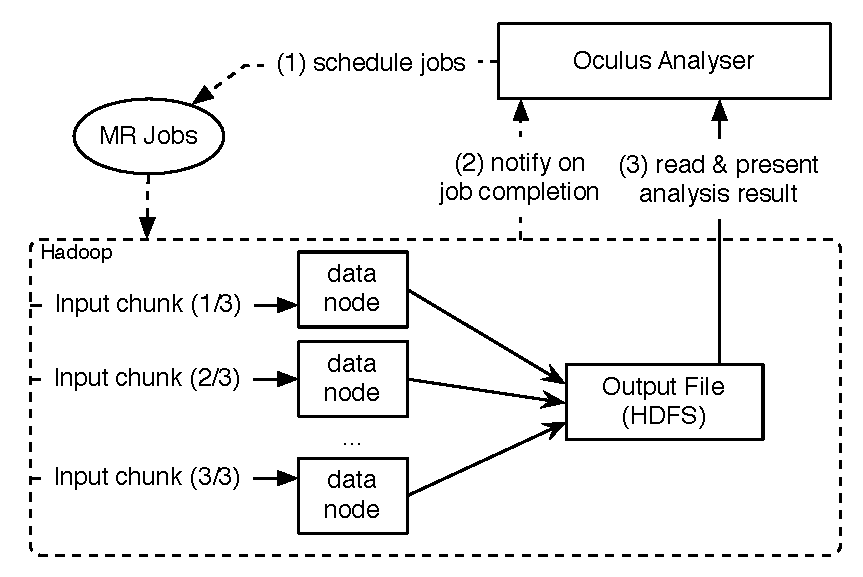
\includegraphics[scale=0.9]{diagrams/analyser-high-level.pdf}
  \caption{When storing a small file in HDFS, it still takes up an entire block. The grey space is not wasted on disk, but causes the \textit{name-node} memory problems.}
  \label{fig:analyser-high-level}
\end{figure}

In step 1 the \textit{job pipeline} is being prepared by the program by aggregating required metadata and preparing the job pipeline, which often consists of more than just one Map Reduce job -- in fact, most analysis jobs performed by Oculus require at least 3 or more Map Reduce jobs to be issued to the cluster. It is important to note that some of these jobs may be dependent on another task's output and this cannot be run in parallel. On the other hand, if a job requires calculating all histograms for all frames of a movie as well as calculating something different for each of these frames -- these jobs can be executed in parallel and will benefit from the large number of data nodes which can execute these jobs.

The 2nd step on Figure \ref{fig:analyser-high-level} is important because Oculus may react with launching another analysis job based on the notification that one pipeline has completed. This allows to keep different pipelines separate, and trigger them reactively when for example all it's dependencies have been computed in another pipeline.

For most applications though the 3rd step in a typical Oculus Job would be to read and present top N results to the issuer of the job, which for a question like ''Which movie is similar to this one?'' would be the top N most similar movies (their names, identifiers as well as match percentage).


% ------------------------------------------------------------------------------------------------------------------------------------------------
\subsection{Defining Map Reduce Pipelines using Scalding and Cascading}
\label{sec:scalding-jobs}
The language and for implementing these processing pipelines used in this thesis was Scalding -- Twitter's home grown Scala DSL, which was already briefly introduced in Section Section \ref{sec:scalding-info}. The choice of using Scalding, and not Hadoop's plain Map Reduce API was mostly dictated by understandability and ease of modifying complicated job pipelines. 

\subsubsection{Comparison of example Job implemented using Plain Hadoop and Scalding}

This section aims to demonstrate what gains using Scalding over Hadoop yields, by showing the smallest possible example of an Map Reduce Job, implemented using both plain Hadoop APIs as well as Scalding. One should remember that Scalding is not a different framework than Hadoop, and in the end it will produce the exact same computations and classes (one instance of an \verb|Mapper| and one instance of an \verb|Reducer|).

The example shown on the below listings is a Hadoop equivalent of what programming languages aim to demonstrate using ''Hello World!'' applications -- it is a minimal piece of code showing the working of the given technology. The task to solve is defined as: ''\textit{Given a huge input text file, count the occurances of each discrete word, and return a summary of these}''. As the aim of Hadoop is to leverage parallel computing, the classic method of implementing this task is to emit tuples of \verb|(word, 1)| for each word, then relying on Hadoops internal mechanisms to group such tuples together by the first value (the \verb|word|), and reducing these into a tuple of \verb|(word, sum(1,1,1,...))| during the Reduce step.

The difference in complexity should be obvious by comparing the Listing \ref{lst:hadoop-mr} which represents the Map and Reduce classes which are used to represent the respectful Map and Reduce functions in the Java API, with Listing \ref{lst:scalding-wc} which is the complete code for a job performing the exact same in Scalding's Scala Domain Specific Language. 

\begin{lstlisting}[caption={Word Count example Job, implemented using plain Java Map Reduce API}, label={lst:hadoop-mr}]
public class Map 
    extends MapReduceBase 
    implements Mapper<LongWritable, Text, Text, IntWritable> {

 private final static IntWritable one = new IntWritable(1);
  private Text word = new Text();

  public void map(LongWritable key, 
                  Text value, OutputCollector<Text, IntWritable> output, 
                  Reporter reporter) throws IOException {
   String line = value.toString();
   StringTokenizer tokenizer = new StringTokenizer(line);
   while (tokenizer.hasMoreTokens()) {
    word.set(tokenizer.nextToken());
    output.collect(word, one);
   }
  }
}

public class Reduce 
    extends MapReduceBase 
    implements Reducer<Text, IntWritable, Text, IntWritable> {

 public void reduce(Text key, 
                    Iterator<IntWritable> values, 
                    OutputCollector<Text, IntWritable> output, 
                    Reporter reporter) throws IOException {
  int sum = 0;
  while (values.hasNext()) sum += values.next().get();
  output.collect(key, new IntWritable(sum));
 }
}
\end{lstlisting}


\begin{lstlisting}[caption={Simplest Scalding job used in Oculus -- each frame perceptual hashing}, label={lst:simplest-scalding-job}]
  Tsv("input.tsv")
    .map('line -> 'word) { line: String => line.split }
    .groupBy('word) { _.count }
    .write(Tsv("output.tsv"))
\end{lstlisting}

As seen on the previous listings, Scalding provides much more concise code, and thanks to this enables developers to focus on the algorithm, and not the boilerplace accompanying these kinds of applications.

\subsubsection{Defining advanced Job Pipelines using Scalding}
Scalding also provides powerful facilities for pipeline building, where by ''Pipeline'' we refer to a series of Jobs that use the output of a previous Job as the input for the next one. It is worth mentioning that this is not something plain Hadoop APIs are able to provide easily, and one would have to implement logic in Jobs that would store the intermediate output in a directory and await the Job's completion, to then manually start the second job (by running it's main method).

Building Pipelines has two major styles in Scalding: explicit ''next Job'' definitions, as well as implicit dependencies on results of Jobs. We will investigate both styles in this section -- starting with the explicit style, as it is more similar to the manual style of doing things.

\begin{lstlisting}[caption={Explicit ''next job'' definition within a Scalding Job class}, label={lst:next-job}]
case class FirstJob(args: Args) extends Job(args) {
  val in = args("in")
  val out = in + ".out"
  
  Tsv(in).read.write(Tsv(out))
  
  def next = Some(SecondJob(Args("--in", out)))
}

case class SecondJob(args: Args) extends Job(Args(out)) { /*...*/ }
\end{lstlisting}

Listing \ref{lst:next-job} shows how one can use Scalding to combine two Jobs using Scalding's DSL. The \verb|SecondJob| depends on the output of the \verb|FirstJob| (which in this case only copies the input to another file on HDFS), since the \verb|next| method is defined within the first Job, we have it's parameters available and can construct the next Job in the pipeline, providing it with it's required \verb|in| parameter. 

\begin{figure}[ch!]
  \centering
  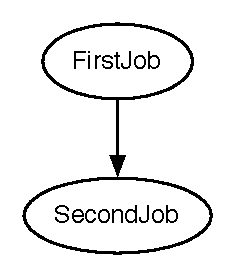
\includegraphics[width=0.3\textwidth]{img/simplest-pipeline}
  \caption{Simplest Job Pipeline, with SecondJob depending on the output of FirstJob (each circle being one Map Reduce Job).}
  \label{fig:simplect-pipeline}
\end{figure}

Such pipeline can be visualised as seen on Figure \ref{fig:simplect-pipeline}, which is an output generated by using the graphviz tool (as in "graph visualization"), applied to a file describing the graph as described in the DOT format. The DOT file corresponding to the graph depicted on Figure \ref{fig:simplest-pipeline} is shown in Listing \ref{lst:simplest-pipeline-dot}. DOT descriptions of pipelines are in common use among profesionals designing such systems, and can also be generated automatically by Scalding -- which is tremendously useful when working with very long pipelines.

\begin{lstlisting}[caption={Textual description of graph on Figure \ref{fig:simplect-pipeline}, using the DOT graph description language.}, label={lst:simplest-pipeline-dot}]
digraph G {
  1 [label = "FirstJob"];
  2 [label = "SecondJob"];
  
  1->2
}
\end{lstlisting}

The second way of building up pipelines is inside one Scalding Job file. Because Scalding's rich set of operations, what may look as simple on the surface (in the pipeline definition) may have to boil down to multiple Map Reduce Job executions. One obvious case that will cause one Scalding Job to produce multiple Map Reduce Jobs is using data from two separate sources and joining them together. It should be noticed that the notion of ''join'' (as known from relational databases) is something both very powerful and very foreign to Hadoop -- as it is only designed to deal with data in a batch-processing fashion. Scalding allows to express join operations trivially in the the definition file, but it's execution actually is quite complicated and forces all the data from one side of the join to be loaded into Mappers participating in the Job's execution.

\begin{lstlisting}[caption={Scalding job, reading data from 2 sources and joining them on dominantColor, producing 3 Map Reduce Jobs}, label={lst:read-and-join-scalding}]
class CompareByDominantColor(args: Args) extends Job(args) {
  // newly analysed video
  val analysedMovieFrames = 
    WritableSequenceFile(input, ("key", "value"))
    .read
    .rename("key", "frame")
    .map(("frame", "value") -> ("dominating", "red", "green", "blue")) { 
        p: (Int, BytesWritable) => calculateHistograms(p._2)
    }
  
  // reference database
  val referenceFrames = 
    HistogramsTable.read
    .rename("dominating", "refDominating")

  // join
  referenceFrames.joinWithSmaller(analysedMovieFrames, 
                                            "dominating" -> "refDominating")
    // operations on joined dataset
}
\end{lstlisting}

Listing \ref{lst:read-and-join-scalding} showcases a simple join operation, which is the core of the algorithms implemented in this thesis. This pipeline definition compiles down into 3 Map Reduce Jobs, because it reads from 2 separate data sources: from a sequence file that we just started processing (this is the movie this job aims to compare to the referece data set), and from the \verb|HistogramsTable| which is the reference dataset containing refernece data calculated previously for all already processed movies in the reference database. The \verb|HistogramsTable| refers to an \textit{HBase Table}, and during the Job's executionw will trigger (in this case) a full-scan over the entire ''histograms'' table stored in HBase - in practice it was feasible to sample down the sample count obtained from HBase, by applying the \verb|.sample(75.0)| operation to the larger data set. Figure \ref{fig:3-pipeline} shows the dependencies as modeled by this definition.

\begin{figure}[ch!]
  \centering
  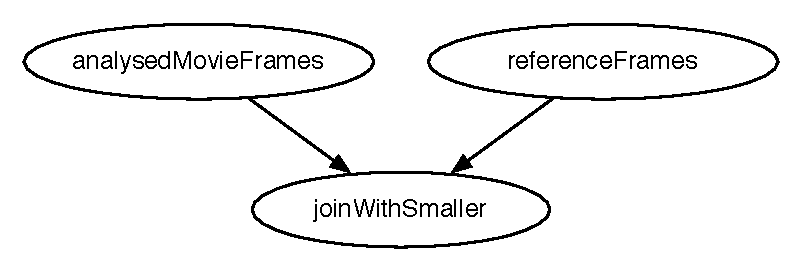
\includegraphics[width=0.75\textwidth]{img/second-simplest-pipeline}
  \caption{Join operation, forcing the Pipeline to consist of 3 Map Reduce Jobs (depicted as circles)}
\end{figure}


The most important thing to notice is that the dependencies, and temporary output directories which are used to pass the data around between the first two Jobs to the 3rd ''Join Job'' were not explicitly modeled, but infered from the use of the \verb|job1.joinWithSmaller(job2, "key1" -> "key2"| operation. Cascading will also take case of deleting these temporary data directories after the job has successuly completed -- another great gain when compared to manual Map Reduce Pipeline implementations.

This section has highlighted how Map Reduce Pipelines can been implemented using Scalding, and have introduced the basic concepts required in order to implement algorithms that can be seen in the following sections.



\subsubsection{Parallel execution and job ordering}
Because a Scalding job (which effectively is an Cascading ''\textit{Pipeline}'') can span multiple Map Reduce Job invocations,
it is important to visualise how many actual Jobs will be submitted to the cluster and also if they can be run in parallel.

In order to visualise how jobs actually will be executed on the cluster Cascading provides a very important option allowing to print the resulting job graph using the widely accepted graph-description language DOT \cite{dot}.

\begin{figure}[ch!]
  \centering
  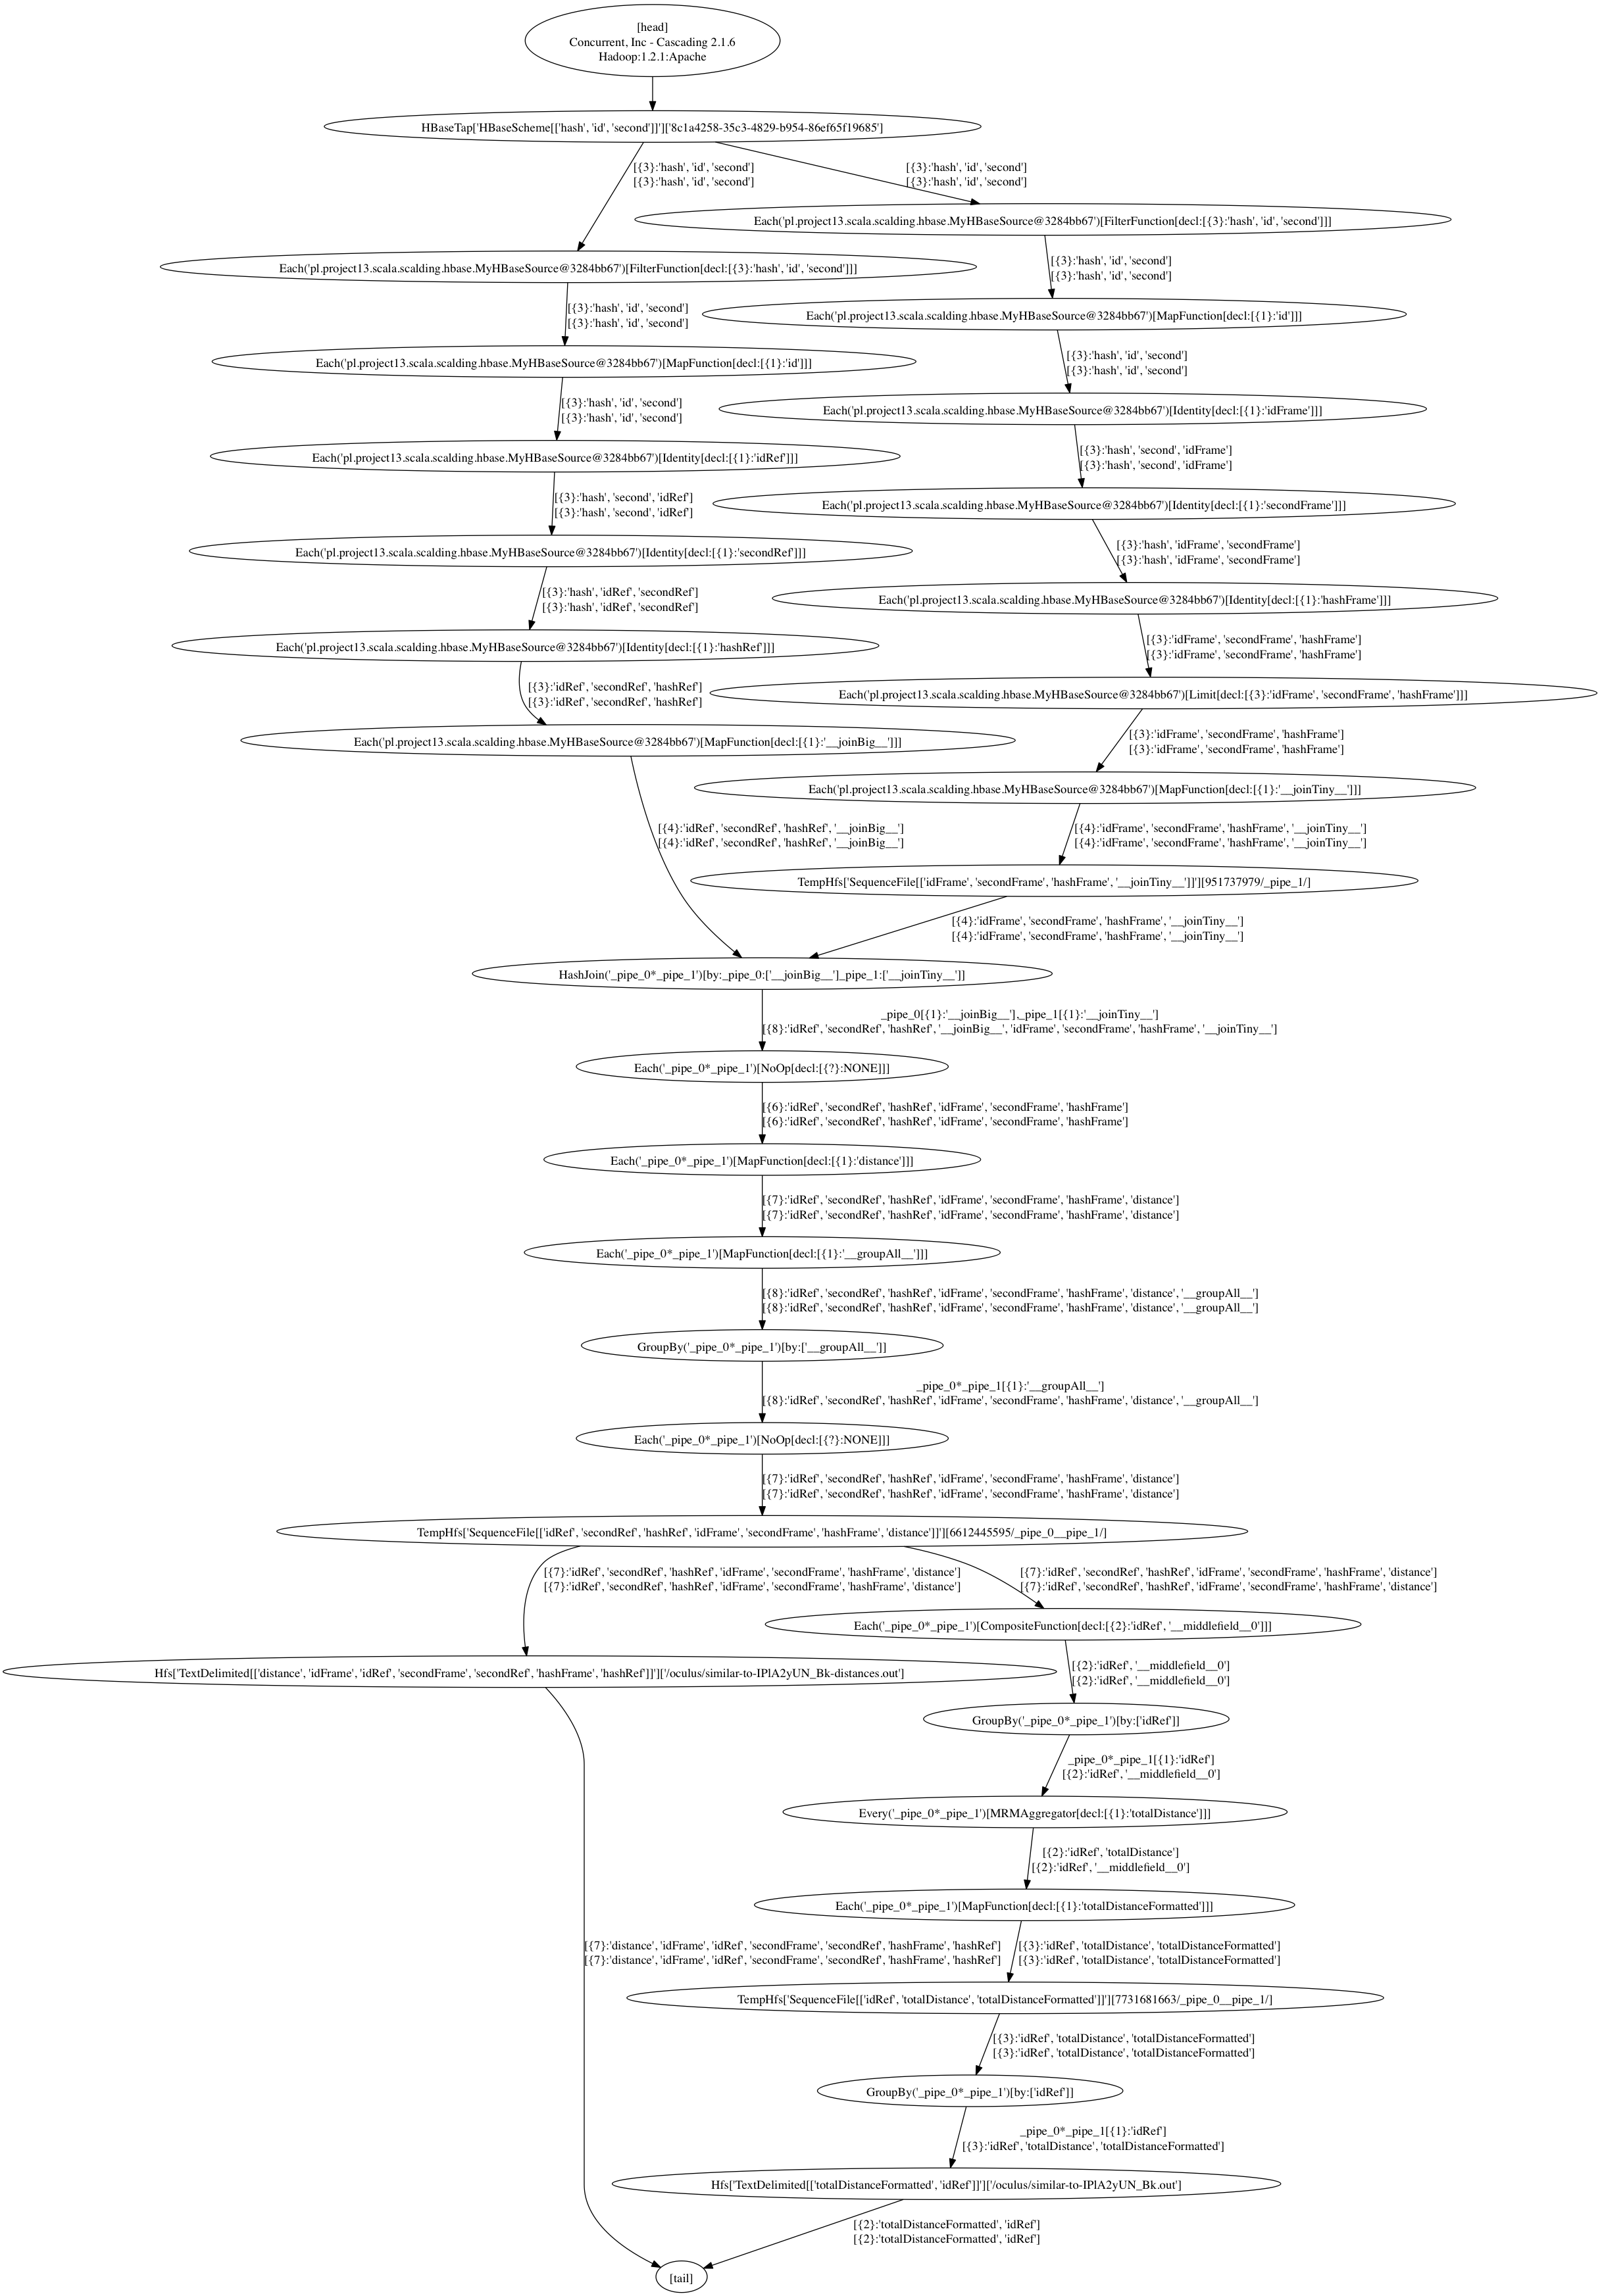
\includegraphics[width=0.9\textwidth]{img/FindSimilarMoviesJob_dot.png}
  \label{fig:find-similar-movies-most-complicated}
  \caption{This flow represents the most longest Pipeline preset in Oculus -- finding which movies are similar to the current one, ordered by ranking. It is constructed from 5 Map Reduce jobs.}
\end{figure}

Figure \ref{fig:find-similar-movies-most-complicated} represents the ''Find similar movies to the given one'' pipeline. Each circle represents an operation (such as emitting a tuple, grouping etc) and lines represent the data flowing through the Map Reduce jobs. It is also clearly visible that this pipeline consists of 5 map reduce jobs, where the 3rd job's input depends on jobs 1 and 2, and only after job 3 has completed jobs 4 and 5 can be executed (in parallel).

Sometimes though it is not easy to determine from this diagram alone how many actual MR Jobs a pipeline has emitted. For this reason we can instruct Cascading to print a DOT file containing the ''steps'', which for the algorithm represented in Listing \ref{lst:find-similar-movies-most-complicated-lst} Figure \ref{fig:find-similar-movies-most-complicated} would look like Figure \ref{fig:find-similar-movies-most-complicated-steps}.

\begin{lstlisting}[caption={Example of Scalding Pipeline exported from the Cascading FlowPlanner using the DOT format}, label={lst:find-similar-movies-most-complicated-lst}]
digraph G {
1  [label = "Hfs['TextDelimited[[UNKNOWN] -> 
               ['refHash', 'frameHash', 'distance']]']['out']"];
2  [label = "Each('_pipe_0*_pipe_1')[NoOp[decl:[{?}:NONE]]]"];
3  [label = "GroupBy('_pipe_0*_pipe_1')[by:['__groupAll__']]"];
# ...
15 [label = "[tail]"];
# ...
    
4->3  [label = "[{4}:'refHash', 'frameHash', 'distance', '__groupAll__']
                [{4}:'refHash', 'frameHash', 'distance', '__groupAll__']"];
3->2  [label = "_pipe_0*_pipe_1[{1}:'__groupAll__']
                [{4}:'refHash', 'frameHash', 'distance', '__groupAll__']"];
1->15 [label = "[{3}:'refHash', 'frameHash', 'distance']
                [{3}:'refHash', 'frameHash', 'distance']"];
2->1  [label = "[{3}:'refHash', 'frameHash', 'distance']
                [{3}:'refHash', 'frameHash', 'distance']"];
# ...
}
\end{lstlisting}


\begin{figure}[ch!]
  \centering
  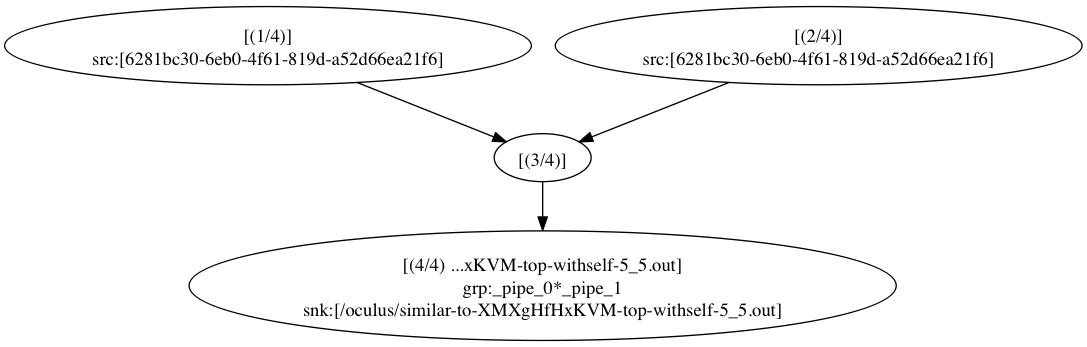
\includegraphics[width=0.9\textwidth]{img/FindSimilarMoviesV2Job-steps_dot.png}
  \label{fig:find-similar-movies-most-complicated-steps}
  \caption{A graph representation of the Map Reduce jobs that have to be run in order to complete the pipeline.}
\end{figure}

The graph represented on Figure \ref{fig:find-similar-movies-most-complicated-steps} displays the same pipeline as Figure \ref{fig:find-similar-movies-most} but on a higher level -- displaying only the order and dependencies of each Map Reduce job. Step \verb|3/4| is easily identifiable as ''groupBy'' here, although from this graph we are unable to determine on what field we're grouping.

\todo{use I, not WE this is not a blog post...}

\todo{needs complete rewrite, slower with examples, show code of the task}
ą





